% !TEX encoding = UTF-8
% !TEX TS-program = pdflatex
% !TEX root = ../tesi.tex

%**************************************************************
\chapter{Descrizione dello stage}
\label{cap:descrizione-stage}
%**************************************************************

\section{Vantaggi per l'azienda}
WebPD trae diversi vantaggi dall'attività di stage curricolare che è stata disposta ad ospitare.\\
\\
Primo su tutti, l'inserimento in azienda, seppur solo per un paio di mesi, di un nuovo membro del personale, mai entrato in contatto con l'azienda. Ciò, in primis, ha permesso di distribuire il carico di lavoro tra più persone, permettendo di accelerare lo sviluppo sui progetti in cantiere. Inoltre, l'introduzione nel team di una persona completamente esterna all'azienda, ha portato un ulteriore punto di vista all'interno del team di sviluppo. Tale punto di vista si è dimostrato utile nel tentativo di risoluzione di alcuni problemi software "cronici" (come la lentezza di esecuzione delle query, problema che verrà descritto nel dettaglio nel prossimo capitolo), permettendo un ragionamento fuori dagli schemi mentali dell'ideatore di tale software.\\
\\
In secondo luogo, ha permesso all'azienda di esplorare nuovi canoni stilistici per alcuni suoi prodotti a costo zero, come nel caso del restyling della homepage del sito CrociereRegalo (descritta anch'essa nel prossimo capitolo), senza quindi il rischio di sacrificare il lavoro (e la retribuzione) di un membro del personale.

\section{Presentazione del progetto}
L'obiettivo di questo stage è permettere a WebPD di completare la riscrittura del sito CrociereRegalo.it. Tale sito, infatti, prima dell'ingresso di Primarete tra le quote di WebPD, era stato realizzato e mantenuto da WebCola, una web agency con la quale Primarete aveva stretto una partnership commerciale, che si è appunto interrotta nel 2015.\\
Secondo gli accordi presi, il sorgente del sito era di proprietà di WebCola, pertanto non è stato possibile per WebPD procedere ad una semplice modifica/aggiornamento di qualcosa già esistente. Il vecchio sito (il cui aspetto è mostrato in Figura \ref{figura:vecchio-sito}), inoltre, non era responsive e, dai dati di Google Analytics è emerso che la maggior parte delle visite avveniva da dispositivi mobili. \\
La problematica maggiore, comunque, si sono rivelati gli accordi presi con le varie compagnie di crociera (MSC, Costa, Royal Caribbean, Celebrity e Azamara): tali accordi, infatti, erano stati presi da WebCola in nome e per conto suo, quindi WebPD si è vista obbligata a ristabilirli.
\begin{figure}[!h] 
	\centering 
	
\includegraphics[width=.9\columnwidth]{stage/webcola_crociereregalo} 
	\caption{Screenshot della versione di CrociereRegalo sviluppata da WebCola}
	\label{figura:vecchio-sito}
\end{figure}\\
Dal 2015 fino ad luglio 2018, WebPD è riuscita a creare un \bookingEngine\hphantom{i}che interagisse con \Gls{api} e \glspl{webservice} forniti da Costa e MSC, permettendo di acquistare una crociera, pagando tramite un payment gateway fornito dal consorzio TVB (Triveneto Bassilichi). La soluzione realizzata, però, aveva grossi problemi di prestazioni (ad esempio la homepage del sito aveva un tempo di risposta medio di 7 secondi, a cui poi doveva essere sommato il tempo di download della risposta, rendering grafico ed esecuzione del codice Javascript presente) e mancava di alcune funzionalità, come la possibilità di vendere tariffe \textit{vuoto per pieno}. Esse non sono altro che posti (cabine) acquistati da un'agenzia viaggi (nel caso in esame, Primarete) ad un prezzo scontato e rivenduti poi ai privati.
\\
Lo stage ha come obiettivo il completamento e l'ampliamento delle funzionalità offerte dal \bookingEngine\hphantom{i}alla base di CrociereRegalo. Più nello specifico, lo stage si propone di svolgere le attività descritte in seguito.

\subsection{Studio di funzionamento del \bookingEngine}
La parte introduttiva dello stage si pone come obiettivo quello di analizzare e capire il funzionamento del \bookingEngine. Infatti quest'ultimo è realizzato tramite il \gls{framework} \textit{Codeigniter}, e, quindi, gode di una struttura delle classi particolare, come anche il modo in cui vengono gestiti gli URL. Inoltre, usando come \gls{DBMS} il software \textit{Microsoft SQL Server}, il linguaggio utilizzato per le interazioni con il database è \textit{Transact SQL}, un dialetto di \textit{SQL}, con il quale è necessario prendere confidenza.

\subsection{Ottimizzazione delle performance del \bookingEngine}
Come accennato precedentemente, il \bookingEngine\hphantom{i}ha grossi problemi di prestazioni. Ciò è dovuto principalmente alla grande mole di dati contenuta nel database, che deve essere interrogato molteplici volte ad ogni richiesta HTTP ricevuta. Gli scopi di questa fase dello stage sono i seguenti:
\begin{enumerate}
	\item Ottimizzare il database in modo che le interrogazioni risultino più veloci. A tale scopo \textit{SQL Server} fornisce una funzionalità chiamata \textit{Database Engine Tuning Advisor} (mostrata in Figura \ref{figura:database-tuning-engine}), che permette, sottoponendole delle query da analizzare, di suggerire la creazione di eventuali indici, in modo da aumentare le performance delle interrogazioni;
	\item Valutare se implementare o meno (e in caso positivo, farlo) un meccanismo di caching dei risultati delle query, in modo da diminuire le interrogazioni al database il più possibile.
\end{enumerate}

\begin{figure}[!h] 
	\centering 
	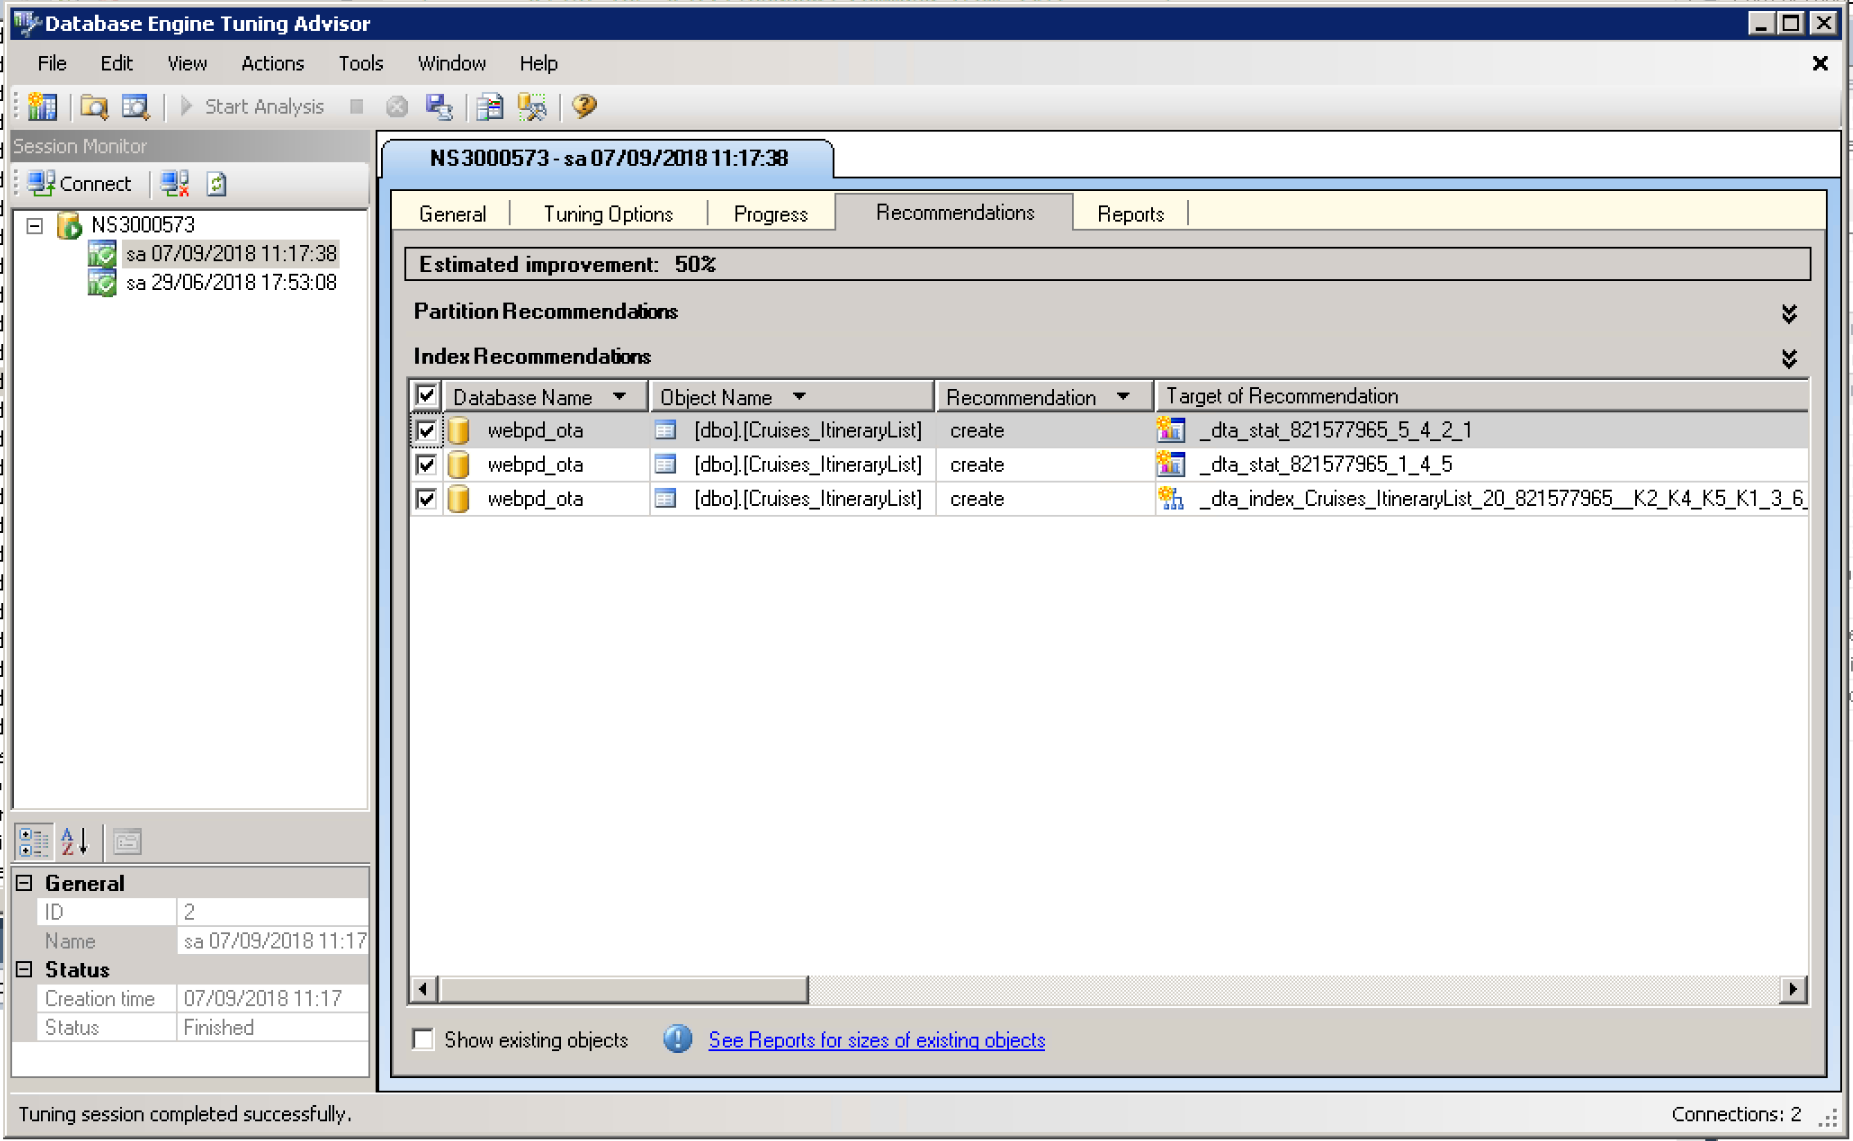
\includegraphics[width=.9\columnwidth]{stage/tuning_query} 
	\caption{Screenshot del tool Database Tuning Engine Advisor utilizzato per l'ottimizzazione delle query}
	\label{figura:database-tuning-engine}
\end{figure}

\subsection{Integrazione delle tariffe \textit{vuoto per pieno}}
Il partner Primarete ha espresso l'esigenza di poter vendere le proprie tariffe \textit{vuoto per pieno} attraverso il \bookingEngine. Come specificato precedentemente, esse sono dei gruppi di cabine acquistate "al buio" da un'agenzia viaggio ad un prezzo scontato (in quanto ne vengono acquistate più di una in blocco), che poi verranno rivendute dall'agenzia stessa ai clienti. Ovviamente, il guadagno dell'agenzia viaggi è rappresentato dalla differenza tra il prezzo di vendita della cabina e quello di acquisto.\\
Il problema è che le cabine associate al \textit{vuoto per pieno}, agli occhi dei \glspl{webservice} delle varie compagnie di crociera, risultano prenotate, quindi non disponibili: è necessario modificare il flusso di prenotazione del \bookingEngine\hphantom{i}permettendo di inserirvi anche i gruppi di cabine acquistate tramite tariffa \textit{vuoto per pieno}, oltre a quelle ancora effettivamente disponibili; tale modifica dovrà essere fatta sia a livello backend che frontend.

\subsection{Aggiunta delle tariffe di un nuovo fornitore}
La versione di CrociereRegalo sviluppata da WebCola integrava, oltre alle crociere di MSC e Costa, anche quelle di Royal Caribbean (e controllate, ovvero Celebrity e Azamara). Lo stage, quindi, si prefigge di ripristinare questa funzionalità anche sulla nuova versione del \bookingEngine\hphantom{i}CrociereRegalo reintroducendo nel flusso di prenotazione le crociere del gruppo Royal, tramite l'integrazione dei \glspl{webservice} forniti da IST (Fibos). Tale integrazione comporterà modifiche sia alla parte frontend che alla parte backend del \bookingEngine


\subsection{Altri interventi minori}
\label{section:altri-interventi-minori}
La fase conclusiva dello stage si prefigge di svolgere interventi minori su CrociereRegalo, per migliorarne la \gls{seo} ed in generale l'accessibilità, soprattutto dai dispositivi mobili.

\section{Obiettivi dello stage}
In fase di definizione contenutistica dello stage, i punti sopra descritti sono stati distribuiti in obiettivi aventi tre livelli di priorità, tenendo conto anche del numero di ore ridotto (circa 310) a disposizione dello stagista, identificati dalle seguenti sigle:
\begin{itemize}
	\item \textbf{Ob} per gli obiettivi obbligatori, vincolanti in quanto obiettivo primario richiesto dal committente;
	\item \textbf{D} per gli obiettivi desiderabili, non vincolanti o strettamente necessari, ma dal riconoscibile valore aggiunto;
	\item \textbf{Op} per gli obiettivi opzionali, rappresentanti valore aggiunto non strettamente competitivo.
\end{itemize}

\begin{longtable}{
		@{}
		>{\raggedright}p{.5cm}
		p{10.5cm}
		>{\raggedleft}p{0.2cm}@{}
		>{\raggedright}p{0.2cm}
		p{8.5cm}
		@{}} 
	\hline
	\multicolumn{2}{|c|}{\textbf{Obbligatori}}\\
	\hline
	Ob1 & Interazione con il database SQL Server attraverso le librerie del \gls{framework} Codeigniter\\
	\hline
	Ob2 & Realizzazione integrazione flat-file di un nuovo fornitore con il Data Exchange del \bookingEngine\\
	\hline
	Ob3 & Aggiunta prodotti e tariffe del nuovo fornitore ai risultati della ricerca lato Front-End del \bookingEngine\\
	\hline
	Ob4 & Esecuzione test e redazione documentazione sul lavoro svolto\\
	\hline
	\multicolumn{2}{|c|}{\textbf{Desiderabili}}\\
	\hline
	D1 & Realizzazione del registro carichi/scarichi tariffe “vuoto per pieno” come	funzionalità lato Back-End del \bookingEngine\\
	\hline
	D2 & Interrogazione web-service in tempo reale per sincronizzare prezzi e disponibilità del nuovo fornitore con il Data Exchange\\
	\hline
	D3 & Realizzazione conferma prenotazione al fornitore come funzionalità lato Front-End del \bookingEngine\\
	\hline
	\multicolumn{2}{|c|}{\textbf{Opzionali}}\\
	\hline
	Op1 & Analisi e realizzazione di nuove funzionalità\\
	\hline
\end{longtable}

\section{Vincoli}
\subsection{Vincoli metodologici}
In accordo con il tutor aziendale, lo stage si è svolto presso la sede dell'azienda. Questa scelta è stata fatta principalmente per due motivi:
\begin{itemize}
	\item agevolare la comprensione, da parte dello stagista, delle dinamiche aziendali e l'interazione con il proponente del progetto CrociereRegalo (WebPD e Primarete hanno l'ufficio all'interno dello stesso palazzo);
	\item favorire al massimo l'interazione tra stagista e tutor aziendale, evitando ritardi di risposta, problematica che invece può avere il \textit{remote-working}.
\end{itemize}
Inoltre è stato deciso che, al raggiungimento di ogni obiettivo prefissato, lo stagista avrebbe dovuto redarre una breve relazione, descrivendo le problematiche affrontate, le scelte adoperate e il risultato ottenuto. Tali relazioni, poi, fungeranno da materiale ausiliario per la presentazione delle nuove funzionalità al proponente.\\
Infine, è stato posto come obbligo che tutto il lavoro prodotto dallo stagista sia sottoposto a versionamento, quindi caricato in un repository Git dedicato, ospitato sul server aziendale.

\subsection{Vincoli temporali}
\label{sec:vincoli-temporali}
Lo stage ha una durata prevista di \textit{310} ore complessive, distribuite in 9 settimane da 34 ore lavorative ciascuna (ad esclusione della prima, da 38 ore). L'orario di lavoro concordato con il tutor aziendale è stato dal Lunedì al Giovedì dalle 09:00 alle 18:30, con 1 ora di pausa pranzo. \\
Prima dell'inizio dello stage è stata definita, nel piano di lavoro, una scansione temporale delle attività con granularità settimanale così definita:
\begin{itemize}
	\item \textbf{Prima settimana}: formazione sulle tecnologie utilizzate dal \bookingEngine\hphantom{i}CrociereRegalo, con particolare attenzione alla libreria \textit{Codeigniter} e al \gls{DBMS} \textit{Microsoft SQL Server};
	\item \textbf{Seconda settimana}: Proseguimento delle attività di formazione iniziate la prima settimana. Ottimizzazione del database tramite gli strumenti forniti da SQL Server;
	\item \textbf{Terza settimana}: Ottimizzazione del sito tramite implementazione della cache delle query. Studio e progettazione dell'aggiunta delle tariffe \textit{vuoto per pieno} al flusso dati del \bookingEngine;
	\item \textbf{Quarta settimana}: Realizzazione, test e redazione di documentazione di quanto progettato la settimana precedente;
	\item \textbf{Quinta settimana}: Studio e progettazione dell'integrazione dati forniti dal sistema FIBOS (Royal);
	\item \textbf{Sesta settimana}: Realizzazione dell'integrazione di navi, porti, itinerari, categorie di cabina e prezzi attraverso interrogazioni schedulate ai \glspl{webservice} FIBOS;
	\item \textbf{Settima settimana}: Realizzazione, test e redazione di documentazione di quanto progettato la settimana precedente;
	\item \textbf{Ottava settimana}: Studio e progettazione dell'aggiunta delle tariffe Royal al flusso di prenotazione;
	\item \textbf{Nona settimana}: Realizzazione, test e redazione di documentazione inerente a quanto progettato la settimana precedente.
\end{itemize}

\subsection{Vincoli tecnologici}
A livello implementativo, l'azienda non ha imposto precisi vincoli, se non quello di aderire il quanto più possibile ai paradigmi di programmazione già preesistenti ed applicare del buon senso a quanto si intende realizzare. Ciò principalmente significa dovrà essere adottato un design pattern \gls{mvc} (il cui schema di funzionamento è mostrato in Figura \ref{figura:mvc}), intrinseco di \textit{Codeigniter}, e cercare di creare del codice che 
sia quanto più manutenibile possibile. Ovviamente, quanto realizzato avrebbe dovuto girare correttamente sull'ambiente di esecuzione già utilizzato, ovvero \textit{PHP 7.1} su \textit{Windows Server 2008 R2}, \textit{IIS} come web server e \textit{SQL Server 2012} come \textit{\gls{DBMS}}.
\begin{figure}[!h] 
	\centering 
	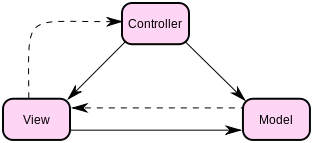
\includegraphics[width=0.6\columnwidth]{stage/mvc} 
	\caption{Schema UML dell'architettura \gls{mvc}. URL: \url{https://bit.ly/2wPfE8E} }
	\label{figura:mvc}
\end{figure}\\

\subsection{La mia scelta}
È da quando ero alle scuole elementari che ho la passione per l'informatica, ed è proprio per coltivare questa passione che ho scelto il cammino di studi che sto portando a termine in questo momento. Sono sempre stato affascinato dalla programmazione web, e il primo linguaggio in cui ho imparato a programmare (da autodidatta, nell'ormai lontano 2012) è stato \textit{PHP}.\\
Dal 2012 ad oggi ho svolto numerosi progetti utilizzando l'accoppiata HTML/PHP, coadiuvata da Javascript e SQL (MySQL). Molti di questi progetti sono stati solo "esercizi di stile", utili per mettermi alla prova, per mettere alla prova quanto imparato e per cercare di ampliare più possibile le mie conoscenze ed abilità nel campo della programmazione. Alcuni progetti, però, sono anche stati adottati e utilizzati da aziende, il ché mi ha regalato non poche soddisfazioni. In ogni caso, ho sempre fatto il programmatore a livello amatoriale.\\
Ho scelto di svolgere questo stage per inserire un nuovo tassello nel percorso di crescita personale che sto intraprendendo: volevo confrontare il mio modo "amatoriale" di lavorare con una way-of-working aziendale. Essendo io già abbastanza familiare con le tecnologie utilizzate da \textit{WebPD}, avrei potuto effettuare un confronto molto diretto tra la metodologia di lavoro aziendale e la mia. 